\documentclass{cubeamer}

\usepackage[french]{babel}
\usepackage[T1]{fontenc}
\usepackage{graphicx}

\title{Protection et gestion des licences}
\subtitle{Présentation - Gestion de projet}
\author{Sami Babigeon, Louka Boivin, Kaci Hammoudi, Alexis Osmont}
\date{\today}
\institute[Université de Rouen]{Master Informatique - 1ère année}

\begin{document}

\maketitle
\cutoc

%
%   Exemple de Plan (mail de Karim)
%
%   Présentation rapide du projet (ie. en une phrase/schéma) Revenir sur les engagements pris initialement auprès du client, 
%   détailler le budget projet (adéquation charge/délais) et le périmètre adressé
%   Ces engagements ont-ils été tenus ? Sinon pourquoi ? Quelles ont été les difficultés rencontrées ?
%   Comment avez-vous surmonté ces difficultés ? Quelles solutions ont été mises en œuvre ?
%   Si le projet était à refaire, quels points d’attention garderiez-vous désormais sous contrôle et comment ?
%   Quels acquis faites-vous suite au projet et gestion de votre projet (ie. vos points forts/points de progression) ?
%   Réussite du projet (ie. retours du client) / ouverture / conclusion


% I   Presentation 
% II  Budget \& Périmètre du projet
% III Engagements 
% IV  Difficultés \& Solutions
% V   Améliorations
% VI  Retour d'expèrience
% VII Conclusion

\section{Présentation du projet}

\begin{frame}{Intitulé}
    \centerline{\textbf{Protection et gestion des licences}}
    \medskip
    \emph{Client :}
    \begin{itemize}
        \item M. Ziadi
    \end{itemize}
    \emph{Objectifs :}
    \begin{itemize}
        \item Protection des logiciels du client
        \item Plateforme de gestion pour le client, de demande pour les utilisateurs
        \item Génération et vérification des licences
    \end{itemize}
\end{frame}

\begin{frame}{Présentation Général}
    \begin{figure}
        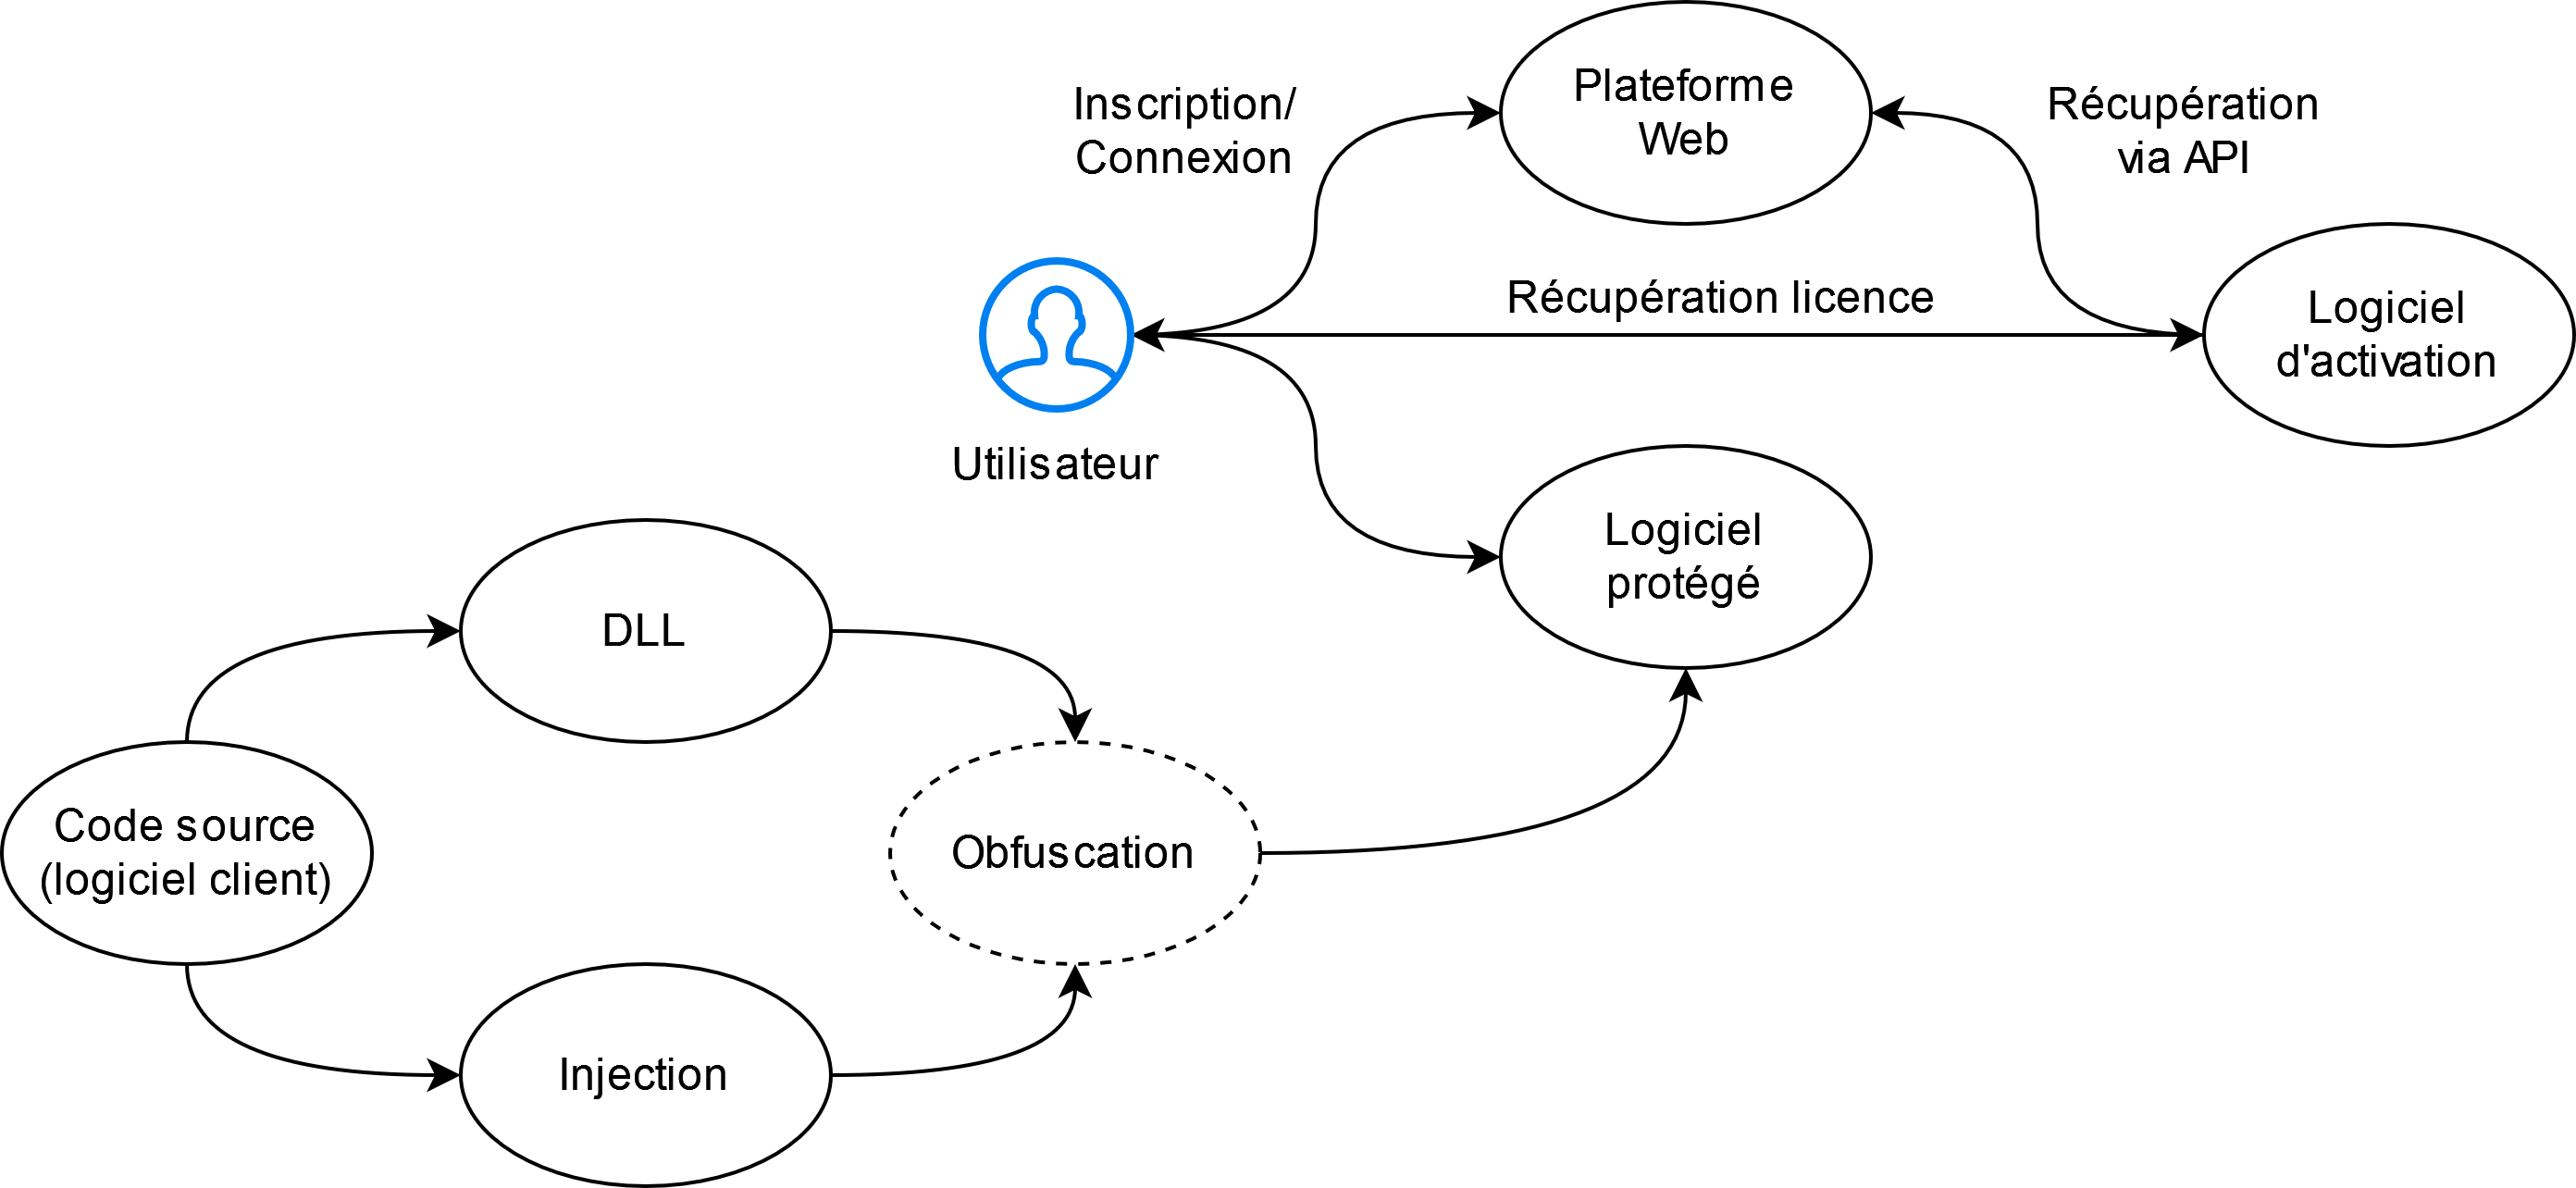
\includegraphics[scale=0.7]{img/general.png}
    \end{figure}
\end{frame}

\section{Engagements}

\begin{frame}{Budget initial}
    \begin{itemize}
        \item 200 heures estimées
        \item 5 membres dans l'équipe
        \item 2 machines virtuelles
      \end{itemize}
 %   \begin{figure}
 %       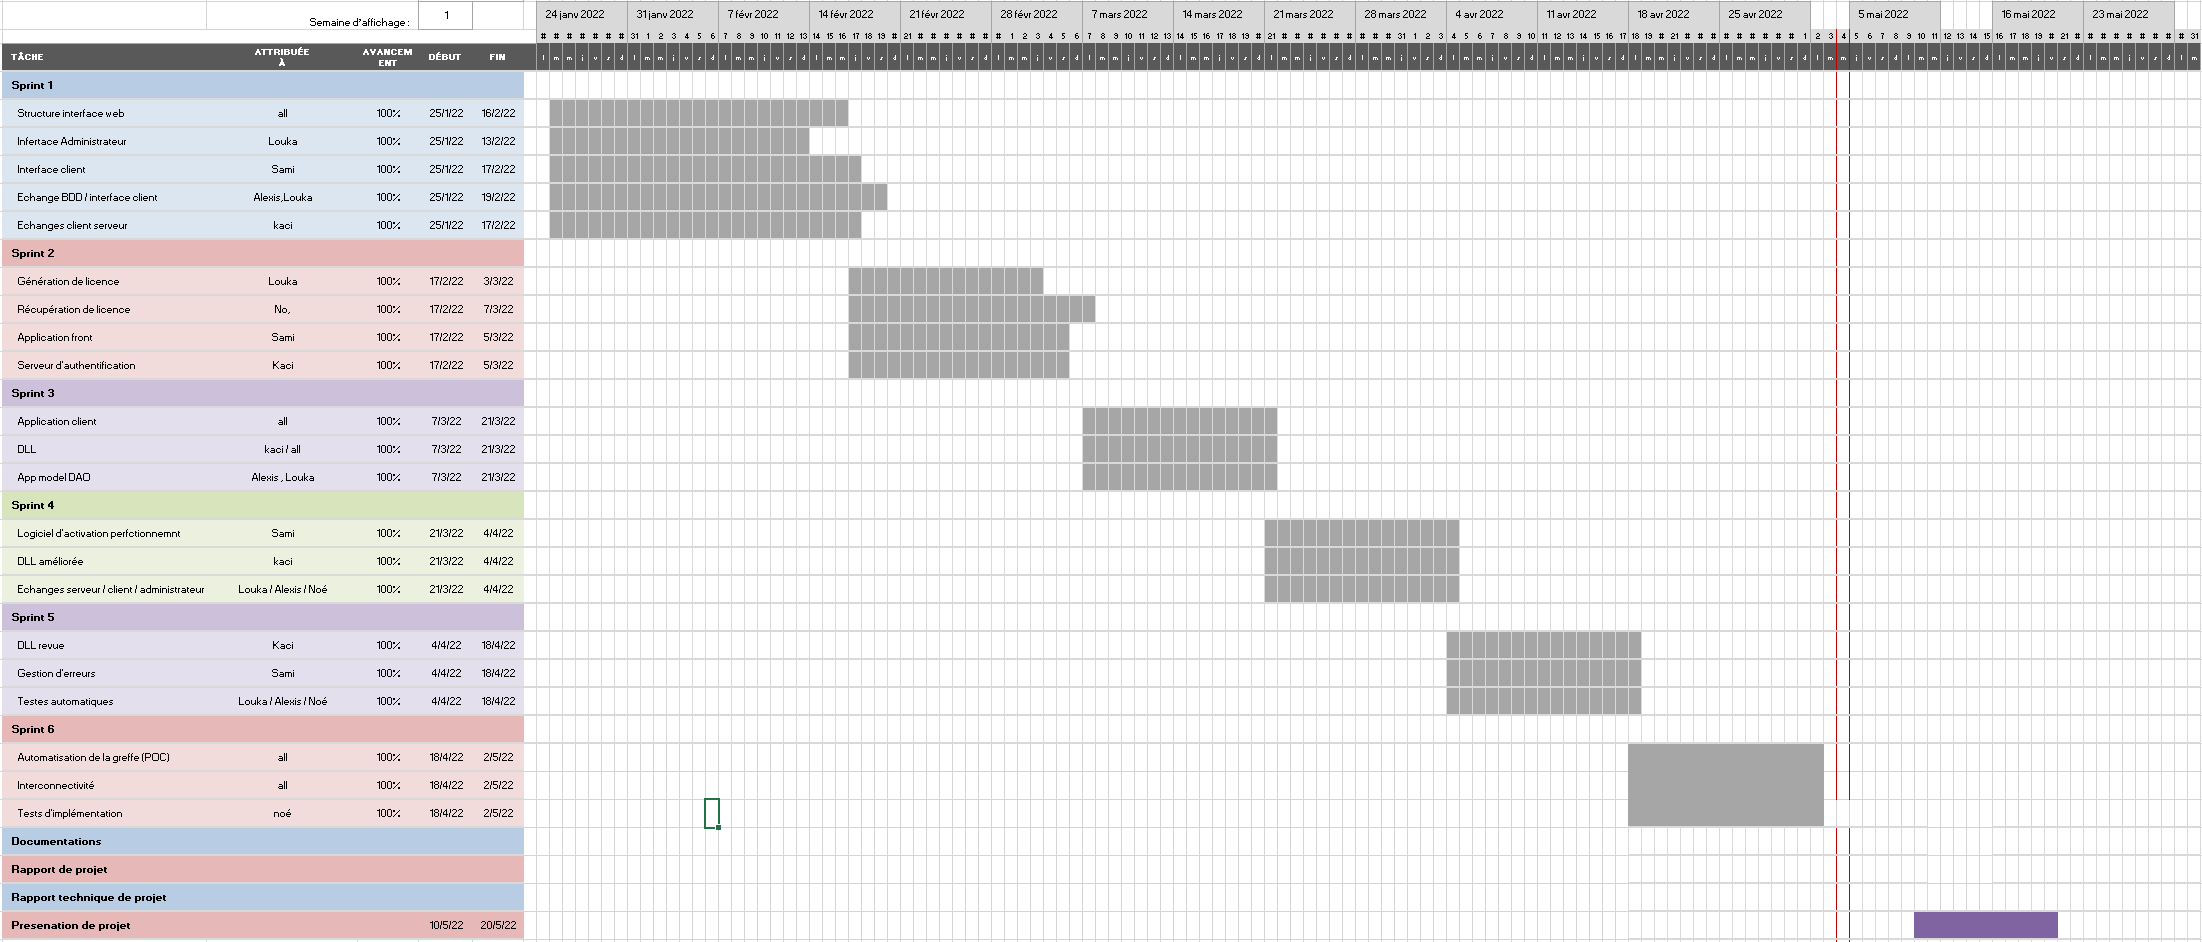
\includegraphics[scale=0.24]{img/Gantt.png}
 %   \end{figure}
\end{frame}

\begin{frame}{Engagements}
    \begin{itemize}
        \item Système de vérification de licence fonctionnel
        \begin{itemize}
        \item Bibliothèque de fonctions
        \item Plateforme web
        \item Logiciel d'activation
        \item Détection de fraude
        \item Obfuscation
        \item Injection de code / greffe 
        \end{itemize}
        \item Documentation
    \end{itemize}
\end{frame}

\section{Engagements tenus}

\subsection{Présentation - Front}

\begin{frame}{Front - Plateforme web}
    \begin{figure}
        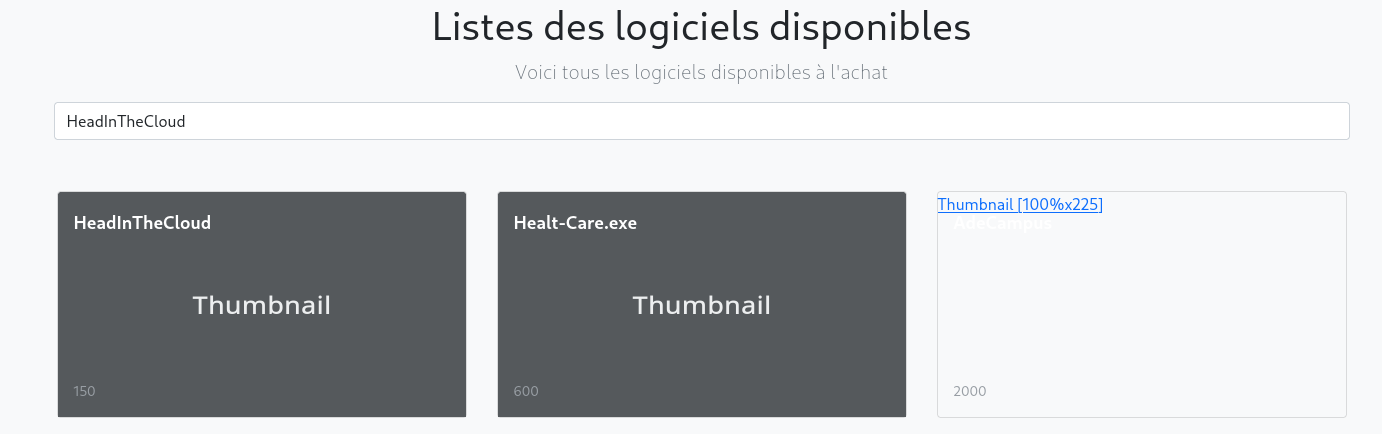
\includegraphics[scale=0.2]{img/web1.png}
    \end{figure}       
    \begin{figure}
        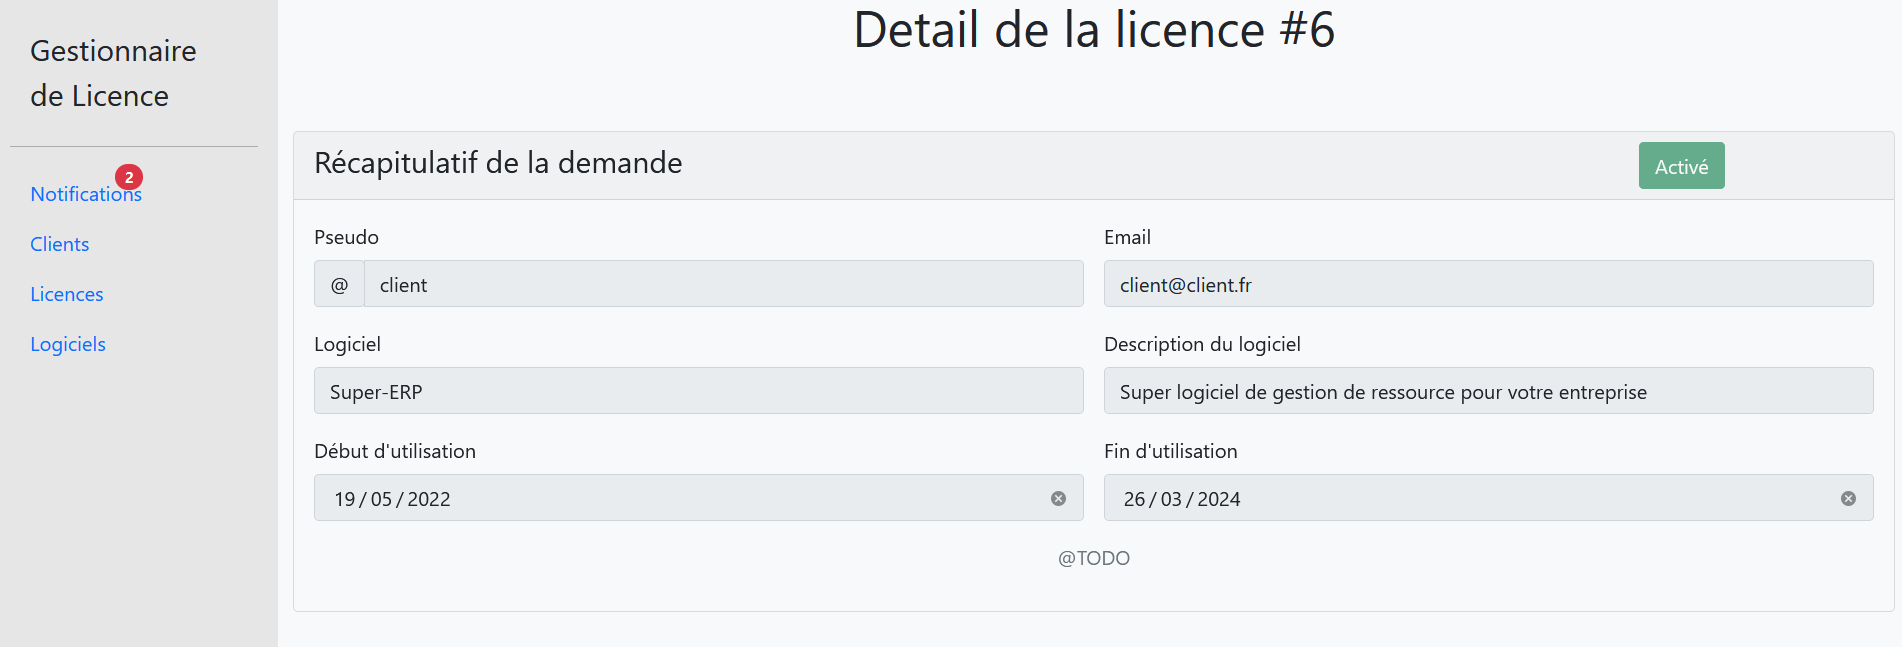
\includegraphics[scale=0.2]{img/web2.png}
    \end{figure}
    \begin{figure}
        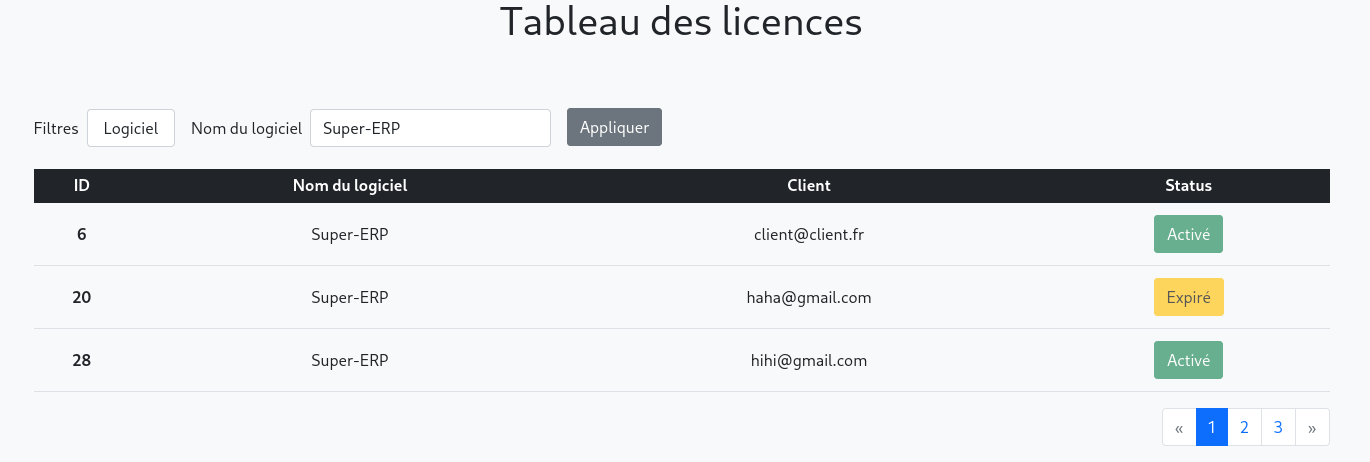
\includegraphics[scale=0.2]{img/web3.png}
    \end{figure}
\end{frame}

\begin{frame}{Front - Logiciel d'activation}
    
\end{frame}

\subsection{Présentation - Back}

\begin{frame}{Back - Génération Licence}
    \begin{figure}
        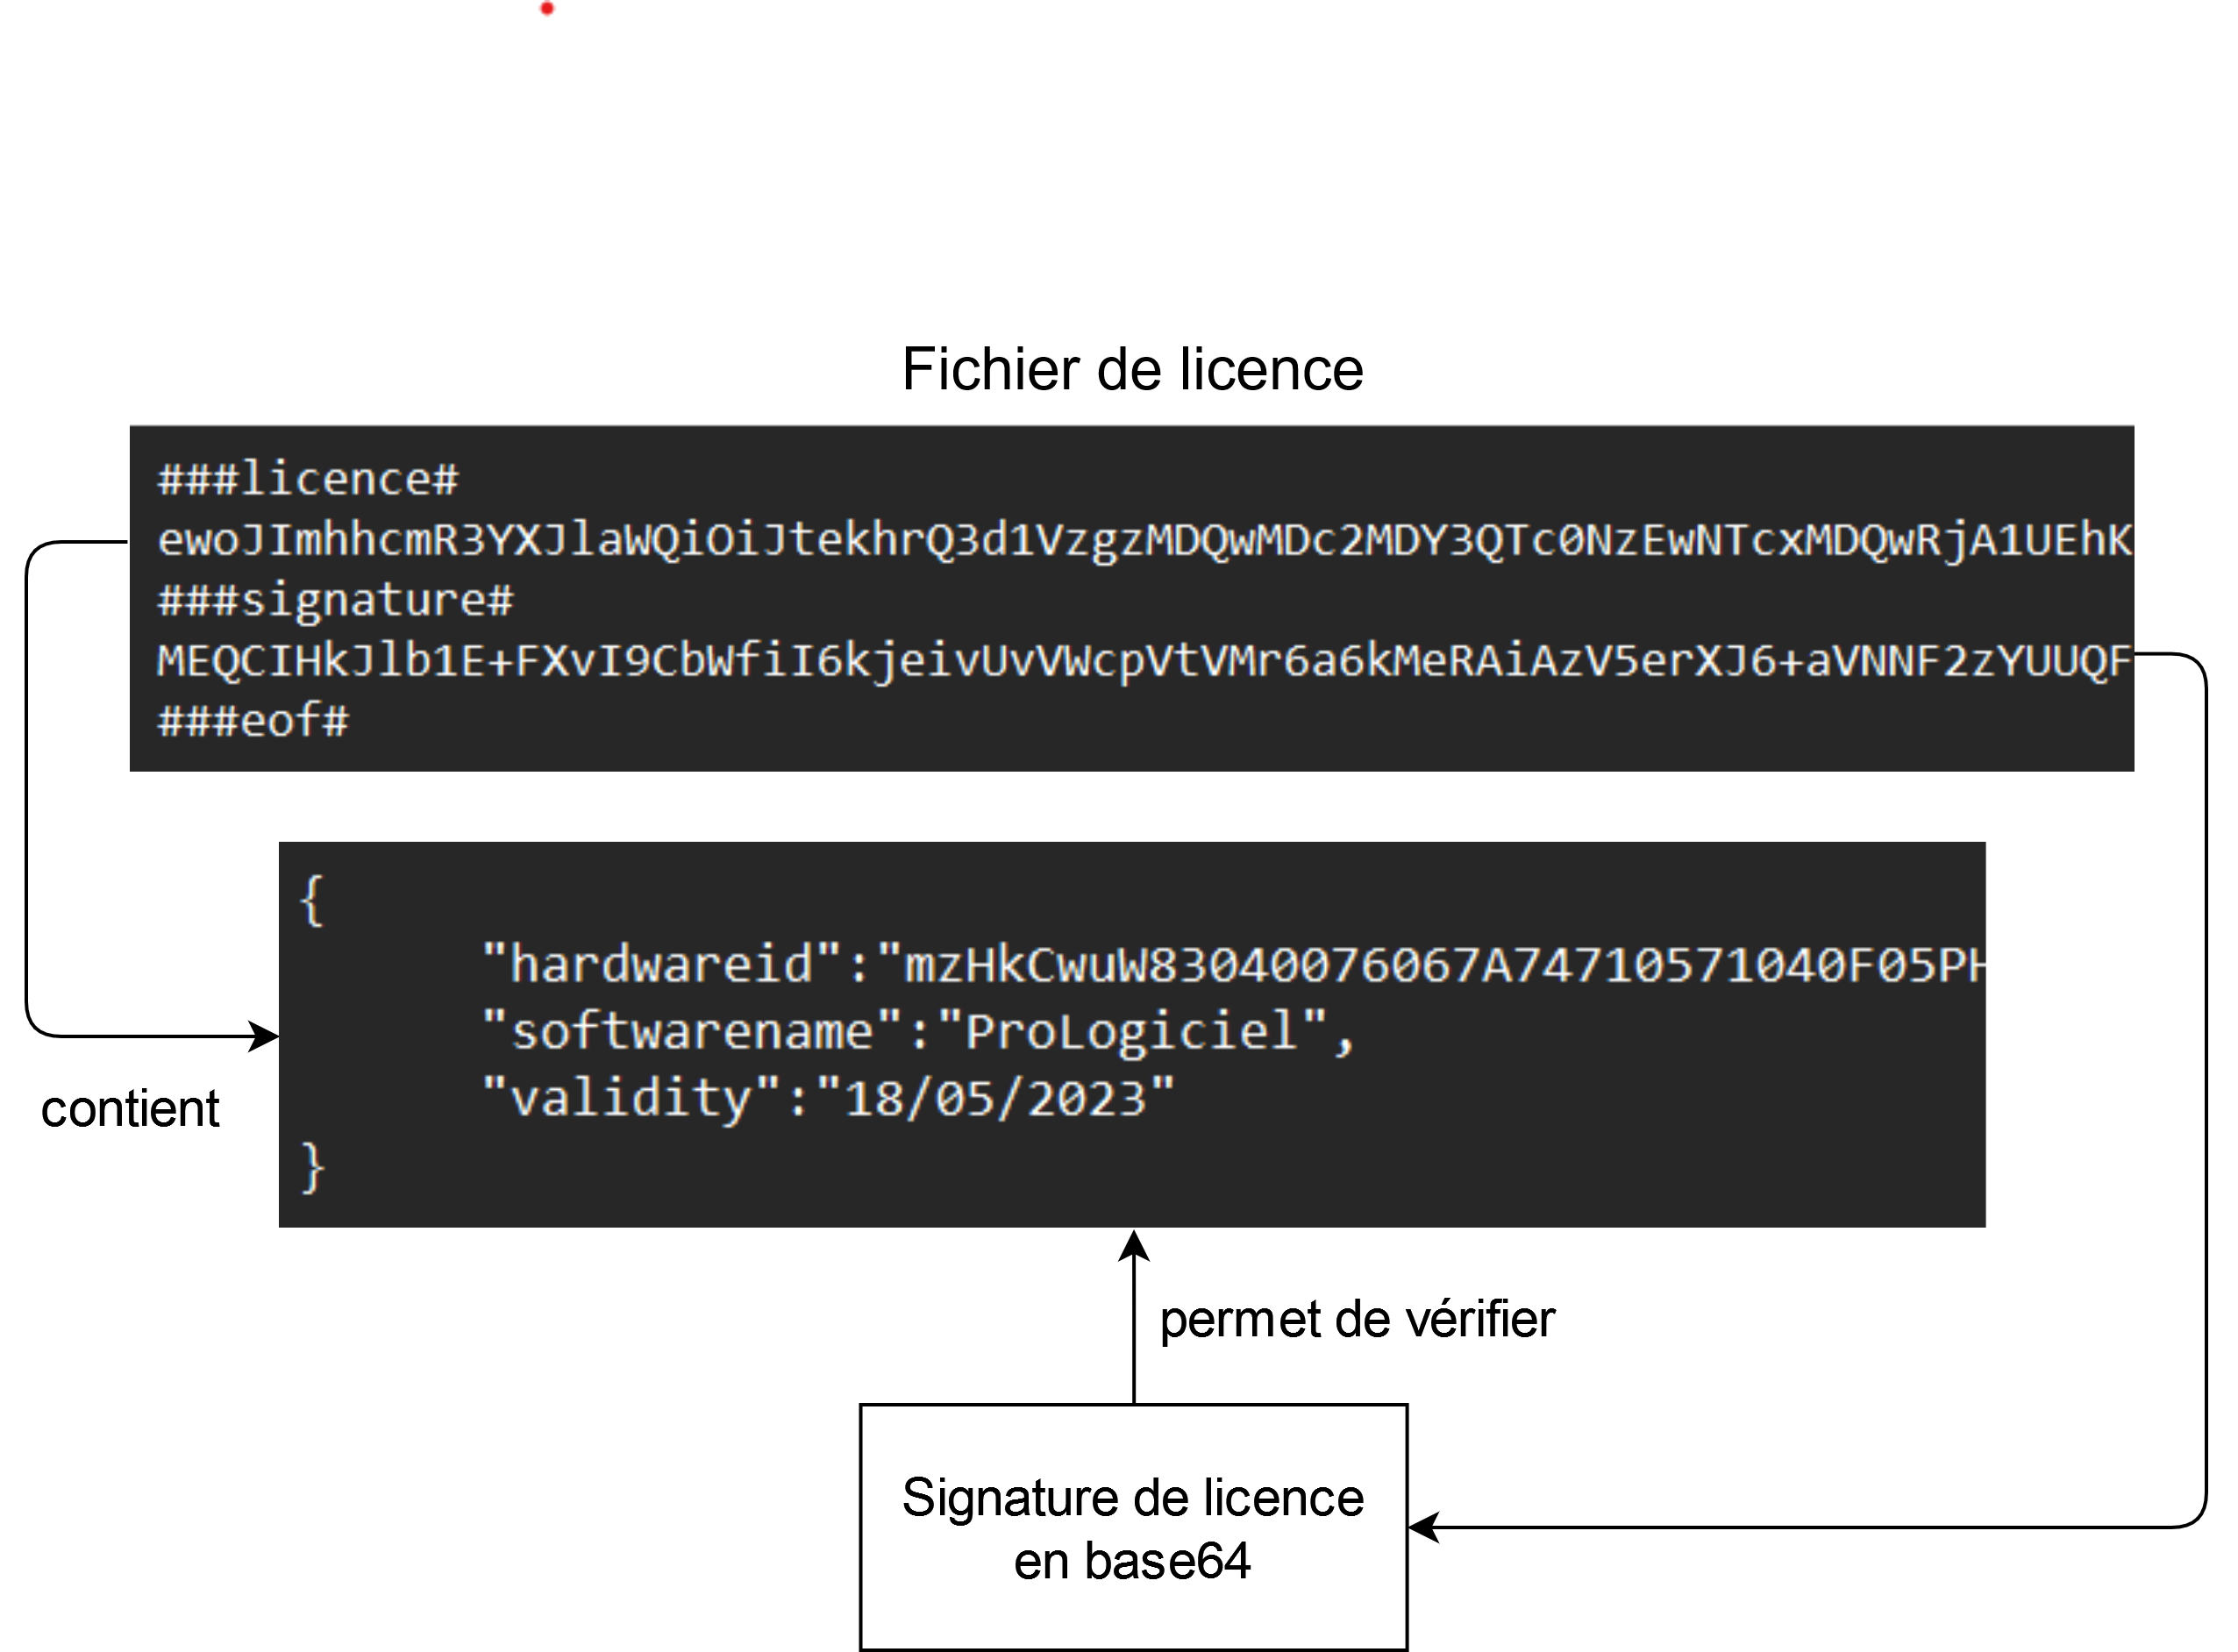
\includegraphics[scale=0.4]{img/licence.png}
    \end{figure}    
\end{frame}

\begin{frame}{Back - DLL}
    
\end{frame}

\begin{frame}{Back - Detection de fraude}
    
\end{frame}

\section{Difficultés rencontrées \& Solutions proposées}

\begin{frame}{Difficultés rencontrées}
    \begin{itemize}
        \item Difficultés Techniques 
              \begin{itemize}
                \item Injection de code
                \item Détection de fraude
                \item Obfuscation
                \item Problème de Réseau
              \end{itemize}
        \item Difficultés Humaines
              \begin{itemize}
                \item Abandon d'un membre du groupe
                \item Communication
                \item Cerner les attentes du client
              \end{itemize}
    \end{itemize}
\end{frame}

\begin{frame}{Solutions proposées}
    \begin{itemize}
        \item Mise en place de protections simple
        \item Configuration réseau statique
        \item Revue du périmètre du projet
        \item Ré-organisation des tâches
        \item Réunion regulière \& utilisation des outils comme \verb:trello:
    \end{itemize}
\end{frame}

\section{Améliorations}

\begin{frame}{Améliorations}
    \begin{itemize}
        \item Revoir les priorités et l'estimation
        \item Mieux écouter les besoins clients
        \item Anticiper les risques
    \end{itemize}
\end{frame}

\section{Retour d'expérience}

\begin{frame}{Retour d'expérience}
    \begin{itemize}
        \item Compétences techniques 
            \begin{itemize}
                \item Programmation Windows 
                \item Connaissances sur les techniques d'injection de code
                \item Mise en place d'un système composé de plusieurs élements
                \item Mise en pratique d'outils cryptographiques
            \end{itemize}
        \item Compétences en Gestion de projets
             \begin{itemize}
                \item Amélioration de nos compétences en gestion de projets \\
                  notamment sur les outils (\verb:git:, \verb:trello:)
                \item Communication \& Organisation
                \item Gestion d'un client
            \end{itemize}           
    \end{itemize}
\end{frame}

\section{Conclusion}

\begin{frame}{Conclusion}
    \begin{itemize}
        \item Première approche de la gestion de projet 
        \item Client satisfait dans l'ensemble
        \item Engagements tenus
    \end{itemize}
\end{frame}

\section{Démonstration}

% Q&A
\begin{frame}[standout]
    \Huge\textsc{Merci de votre écoute}
    \vfill
    \LARGE\textsc{Questions ?}
\end{frame}

\end{document}

